\documentclass[12pt]{article}

% USEPACKAGES
\usepackage[margin=2.5cm]{geometry} % Change border margins.
\usepackage[titles]{tocloft} % Table of Contents, manual add.
\usepackage{mcode} % Load matlab code into LaTeX.
\usepackage[parfill]{parskip} % Removes indents
\usepackage[hidelinks]{hyperref} % Clickable links in PDF.
\usepackage{fancyhdr}
\usepackage{graphicx}
\usepackage{epstopdf}
\usepackage{float}
\usepackage{amsmath,amssymb,amsthm,multirow,algorithm,algorithmic,amsfonts}
\usepackage{gensymb}
\usepackage[square,numbers,comma,sort&compress]{natbib}
\usepackage[toc,page]{appendix}
\usepackage[final]{pdfpages}
\usepackage{afterpage}
\usepackage{mdwlist} % Compact lists (itemize*)
\usepackage{fixltx2e}
\usepackage[table]{xcolor}
\usepackage{expl3}

\usepackage{lscape}
\usepackage{rotating}

% PAGESTYLE
\pagestyle{plain}

% COMMANDS
\newcommand{\HRule}{\rule{\linewidth}{0.04cm}}
\renewcommand{\abstractname}{{\Large Summary}}
\renewcommand{\cftsecleader}{\cftdotfill{\cftdotsep}}
\setlength{\parskip}{12pt plus8pt minus6pt}

% ENVIRONMENTS
\newenvironment{drawing}


\begin{document}
% Titlepage
\begin{titlepage}
\begin{center}

% Upper part of the page
\textsc{\LARGE Delft University of Technology}\\[0.3cm]
\textsc{\Large Design Synthesis Exercise}\\[0.5cm]

% Title
\HRule \\[0.4cm]
{\Large \bfseries Design of a Controllable Inflatable Aeroshell}\\[0.2cm]
{\Huge \bfseries Project plan}\\[0.2cm]
\HRule \\[1.2cm]

% Image
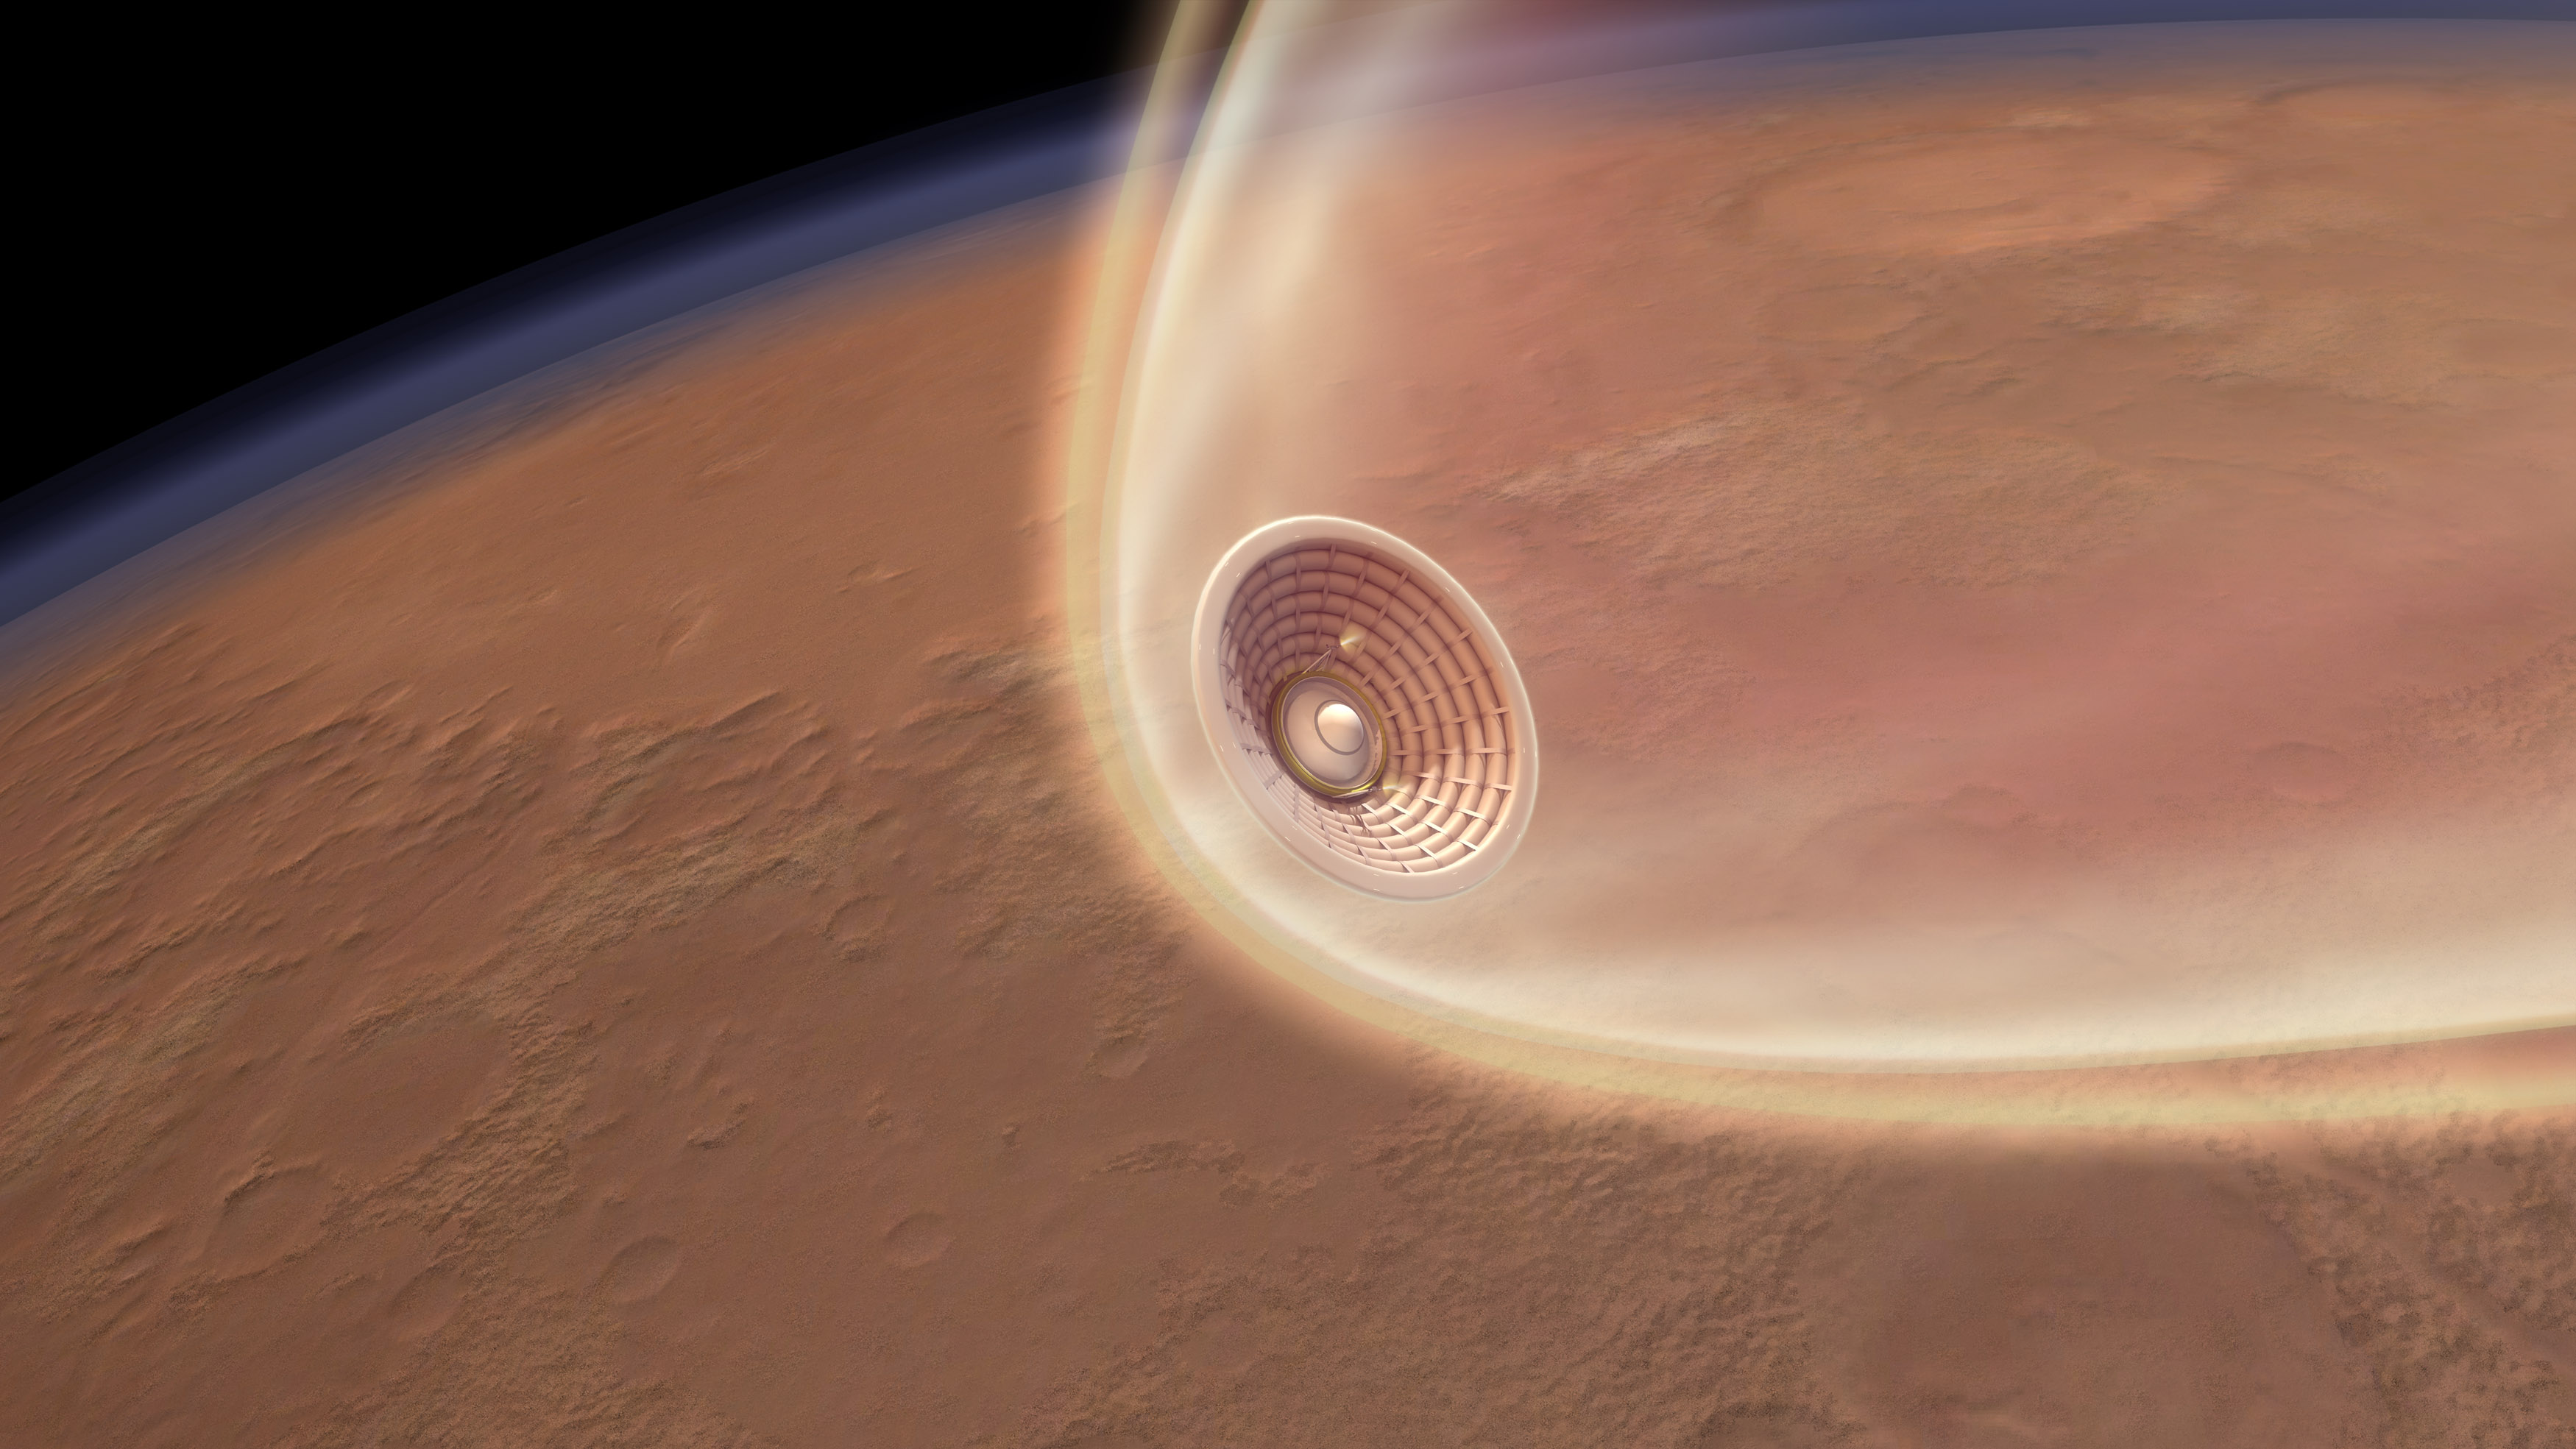
\includegraphics[scale=0.4]{./Titlepage/coverpicture}\\[1cm]

% Author
S. Balasooriyan \\
B. van Dongen \\
D.D. Hage \\
T. Keijzer \\
G. van Koppenhagen \\
L. Mathijssen \\
J. Meulenbeld \\
A. van Oostrum	\\
S. van Schie \\




\vfill

% Date
\begin{large}\today \end{large}

\end{center}
\end{titlepage}
\pagenumbering{roman}
% Summary
\newpage
\section*{Summary}\label{cha:summary}


Inflatable aeroshell concepts hold the key to what is currently unattainable for interplanetary human spaceflight. In the wake of current \acrfull{nasa} investigations on the feasibility of inflatable decelerators for hypersonic guidable re-entry, this study focuses on Mars entry of a payload mass of at least 9000 [kg] using an inflatable aerodynamic decelerator of at most 1000 [kg]. Such a solution provides a large economical advantage over conventional solutions by maximizing payload-carrying capability through a light-weight device less burdened by launcher size considerations. This Mid-term Report gives an overview of conceptual design activities, comprising aerodynamic, structural, thermal, astrodynamic and control tool development and analysis, leading up to concept selection in a trade-off.
\newline
\newline
To aid in the conceptual analysis, design and selection process and to provide a basis for further design efforts after concept selection in the \acrfull{mtr} a number of tools have been developed with the following purposes:
\begin{itemize}
\item A tool for parametric structural mass modelling
\item A modified Newtonian flow aerodynamic tool for the characterisation of aerodynamic and aerothermal behaviour
\item A thermal model for \acrfull{tps} sizing and analysis
\item An astrodynamic tool with an implemented control system for trajectory control
\end{itemize}

Concepts were selected for trade-off as the outcome of a structured \acrfull{dot} on the basis of concept shape. Shape is chosen to have a leading factor due to its importance in the aerodynamic and trajectory performance, which directly flows down to thermal, structural and control performance. The initial concept selection yielded five concepts for trade-off: a conventional capsule concept and four inflatable concepts, namely stacked toroid, tension cone, trailing ballute and isotensoid configurations. To reflect concept capability of meeting customer demand, the following concept aspects have been evaluated as trade-off criteria: decelerator mass, development risk, vehicle stability and deceleration time.
\newline
\newline
The first trade-off criterion, decelerator mass, is essential since it is highly desirable that payload-carrying capability is maximised. To make full use of the launcher carrying capability, a decrease in decelerator mass allows for an equal increase in payload mass. To this end, structural, thermal and control system mass were estimated as the distinguishing mass components between concepts. 

The lowest structural mass was achieved by the stacked toroid configuration, followed upon closely by the isotensoid, tension cone and trailing ballute configurations (an estimated 110, 168 and 221 \% of stacked toroid structural mass respectively). \acrfull{tps} and control system mass analysis yielded estimates of 100, 84, and 76 \% and 100, 67, and 96 \% of stacked toroid mass for tension cone, trailing ballute and isotensoid configurations respectively. This yields total decelerator masses of 116, 113 and 88 \% of stacked toroid mass, based on weight contributions of 20, 50 and 15 \% by structure, \gls{tps} and control system mass. A mass analysis for the rigid concept showed a decelerator mass well in excess of the imposed maximum 1000 [kg], 2945 [kg] for thermal and structural mass alone.
\newline
\newline
The second trade-off criterion, development risk, is essential since concepts with a low \acrfull{trl} incur higher schedule and cost risks. The tried-and-true rigid solution thereby has \gls{trl} 9, while inflatable concepts are notably less explored. A recent surge in interest in inflatable concepts by \gls{nasa} and a consistent development program has brought the stacked toroid configuration to \gls{trl} 7. The other three inflatable concepts are less explored, having only undergone a selected set of tests and research and hence designated \gls{trl} 4. The trailing ballute concept is deemed to have a higher development risk still, by its only feasible control option being a relatively underdeveloped one, namely morphing, reflected by \gls{trl} 2.
\newline
\newline
The third trade-off criterion, deceleration time, is evaluated as a shorter entry time is desirable. As ground operations are to be maintained at fully capacity during entry, a shortening of entry time will alleviate costs incurred. Moreover, physical taxation of human payload is decreased as deceleration time is decreased.  A decreased deceleration time is obtained by better controlability of the spacecraft. To this end, concepts were evaluated for their performance in lift to drag ratio. The rigid concept was found to be able to provide a relatively high lift to drag ratio which consequently will result in short deceleration time. The stacked toroid, tension cone and ballute concept were found to provide an adequate value and finally the isotensoid deceleration performance was found to be poor in this trade-off criteria.
\newline
\newline
It is preferable that concepts are stable, since a stable vehicle will counteract perturbations to move back to its equilibrium condition and its intended trajectory. To this end, static stability was investigated by aerodynamic analysis. Stacked toroid, tension cone and ballute were found to be stable; the rigid concept is neutrally stable and the isotensoid is unstable. The first three therefore perform well, the rigid concept performs adequately and performance of the isotensoid is deficient for the fourth and final trade-off criterion.
\newline
\newline
On the basis of the analysis presented in this Mid-Term Report, design options and their prospective advantages and disadvantages are presented to the customer at the \gls{mtr}. Hereafter dialogue is entered to yield a final concept for preliminary design that satisfies customer demands. The next phase then commences with a more detailed analysis and design of the selected concepts, aided by tool enhancement. This phase entails a more refined orbit optimization, aerodynamic shape determination and structural and \gls{tps} design and sizing. A structured approach to this next phase is facilitated by breaking down future work, resource allocation and is aided by an interface definition given in this report to define the interaction of subsystems within the design process.

% Table of contents
\newpage
\tableofcontents
\addtocontents{toc}{\protect\contentsline {section}{Summary}{i}{}}

% Chapters
\newpage
\pagenumbering{arabic}
\section{Introduction}
\label{cha:introduction}
Before human interplanetary spaceflight can be achieved technological gains have to be made in several fields. One of these fields comprises hypersonic deceleration systems. Significant weight gains are expected to be possible by using inflatable aeroshells. However, the development of a controllable inflatable aeroshell is very complex and consists of many different disciplines. To reduce the complexity of designing such a system first a \acrfull{pp} was made. Following that a \acrfull{br} was produced, in order to survey the current technology state and knowledge on this subject. Now a \acrfull{mtr} report is made in order to perform a concept trade-off. 

The purpose of this report is to present several concepts for a controllable inflatable aeroshell and to determine which concept is best suited for performing the design mission. First the group organisation for the period between the \acrlong{mtr} and \acrlong{fr} is discussed in chapter \ref{ch:wdd}, including individual and group tasks and work packages. A \acrfull{wbs} is made, together with a \acrfull{wfd} and Gantt chart. Secondly the approach with respect to sustainable development is presented in chapter \ref{ch:sustain}. Thirdly the \glspl{dot} are used in chapter \ref{ch:options} to generate several system concepts. These concepts will be analysed with tools from several different disciplines. These consist of an astrodynamics \& control tool, as well as tools for concept mass estimation, aerodynamical characteristics and thermodynamic behaviour. The development, verification, validation of these tools is discussed in chapters \ref{ch:astrocontrol}, \ref{ch:strucmass}, \ref{ch:aero_analysis} and \ref{ch:thermtool} respectively. These chapters also show the results obtained from analysing the proposed system concepts. After the tool development and concept analysis the risk inherent to each system concept is considered in chapter \ref{ch:riskestimation}. This will be done by making a risk map for each concept. Finally the concept trade-off will be performed in chapter \ref{ch:tradeoff}, based on results of the analyses conducted in the previous chapters. The result of this is a complete trade-off matrix, after which the customer will be able to select the preferred concept based on the weights they attach to each trade-off criterion.
\section{Project description}\label{cha:project_description}%Notes: Stand alone, consise and do not explain anything.
This chapter provides an overview of the project. In section \ref{subsec:missionframework}, an introduction to the mission and a historical perspective is given, while the top-level system requirements are stated in section \ref{subsec:systemrequirements}.

\subsection{Mission framework} 
\label{subsec:missionframework}
Ever since successful manned missions to the moon, the next interest has lain in a manned mission to extraterrestrial locations. Entry in the atmosphere of, for example Mars, induces great aerodynamic loads which lead to high thermal and structural loads on the structure. Where a spacecraft structure can be designed for very high loads, the human body is limited in the loads it can endure. 

The mission need statement may thus be formulated as: Design a sysytem to perform an entry on Mars while keeping loads within the limits of what the human body can endure while adhering to launch constraints in the form of launcher fairing and entry mass. Since Mars is the most challenging case for such a mission, it is used as mission case for the project at hand. \cite{projectguide}

<<<<<<< HEAD
A very promising design to perform such an entry is an inflatable guidable entry vehicle using a \gls{hiad}, since it allows a decrease in spacecraft mass and respects fairing dimensions in stowed condition. Previous missions comparable to the to-be-developed mission have been performed by \gls{nasa}, demonstrating the controllability of an inflatable aeroshell, as early as in the 1960s. Multiple concepts were developed: a chute that is held under tension with a pressurized toroid that was attached to the structure in one case and trailed the spacecraft using a tow in the other case. These concepts were developed to allow re-entry on Earth and Mars, but were discontinued when problems arose during deployment and contemporary parachute technology proved sufficient for the design goals back then. \citep{hiadhistory}
A pressurized cone containing multiple toroids is another option that receives considerable attention from NASA in the form of three missions performed in the last six years. A fourth mission is planned in 2016. The first IRVE mission spacecraft failed to deploy it's inflatable structure. The second mission (IRVE-II), though, was a success, and showed the potential for this deceleration method. The third mission (IRVE-3) tried approximately the same concept from a higher altitude, while THOR is scheduled to provide more insight in controllability of the spacecraft. \cite{irve2,irve3,thor} A comparison of key design parameters of these missions can be found in Table \ref{tab:hiadcomparison}.
These tests are now in the spotlight since interplanetary missions involving humans are on the program, with the NASA planning to have humans on Mars by 2030.\footnote{URL: http://www.space.com/24268-manned-mars-mission-nasa-feasibility.html. Accessed: 22 April 2015} Since transporting humans puts constraints on maximum deceleration, the present project may provide means to decelerate the interplanetary spacecraft with lower accelerations while being a more light-weight solution than current thruster designs.
=======
A very promising design to perform such an entry is an inflatable guidable entry vehicle using a \gls{hiad}, since it allows a decrease in aircraft mass and respects fairing dimensions in stowed condition. Previous missions comparable to the to-be-developed mission have been performed by \gls{nasa}, demonstrating the controllability of an inflatable aeroshell, as early as in the 1960s. Multiple concepts were developed: a chute that is held under tension with a pressurized toroid that was attached to the structure in one case and trailed the spacecraft using a tow in the other case. These concepts were developed to allow re-entry on Earth and Mars, but were discontinued when problems arose during deployment and contemporary parachute technology proved sufficient for the design goals back then. \citep{hiadhistory}
A pressurized cone containing multiple toroids is another option that receives considerable attention from NASA in the form of three missions performed in the last six years. A fourth mission is planned in 2016 \cite{ivre,irve2,irve3,thor}. Every next mission shows another aspect with respect to feasibility, controllability and ability to control the maximum deceleration achieved during re-entry. A comparison of key design parameters of these missions can be found in Table \ref{tab:hiadcomparison}.
These tests are now in the spotlight since interplanetary missions involving humans are on the program, with the NASA planning to have humans on Mars by 2030.\footnote{URL: http://www.space.com/24268-manned-mars-mission-nasa-feasibility.html. Accessed: 22 April 2015} Since transporting humans puts constraints on maximum deceleration, the present project may provide means to decelerate the interplanetary spacecraft with lower accelerations while still being a light-weight solution.
>>>>>>> da416cf3e22a6b8cb5745723cef9bd4e4c940c20

% Three designs have been made and tested on earth by NASA and the next will be launched in 2016 \cite{irve,irve2,irve3,thor}. These designs show the feasibility of using this method to do a re-entry. 
The top-level requirements of this mission are almost entirely based on two mission needs. Firstly, there are humans on board the (re-)entry vehicle. Secondly, existing launchers have to be used . As these needs are of utmost to the project and it has therefore been decided to include them in the project objective statement. The objective of this project is thus: design a controllable inflatable (re-)entry vehicle for hypersonic guided Mars entry of human class spacecraft using available launchers with nine persons in ten weeks time.

\begin{table}[ht!]
\vspace{-20mm}
	\caption{Comparison of recent HIAD missions}% CAPTION HERE !
		\begin{tabular}{|p{0.28\textwidth}|p{0.12\textwidth}|p{0.15\textwidth}|p{0.15\textwidth}|p{0.21\textwidth}|} % MAKE SURE THAT THE TOTAL WIDTH IS 0.95\textwidth!! (that way its exactly the textwidth.... haha) 
			\hline

       Mission parameter   &       Unit &     IRVE-2 \cite{irve2} &     IRVE-3 \citep{irve3,thor} & THOR (predicted) \citep{thor} \\
			\hline \hline

Launch date &          - & 17-08-2009 & 23-07-2012 &       2016 \\
			\hline

      Mass &         kg &    124.6kg &        280 &        315 \\
			\hline

Shell diameter &          m &       2.93 &       2.93 &        3.7 \\
			\hline

Shell angle &     deg &         60 &         60 &         70 \\
			\hline

    Apogee &         km &        218 &        469 &    200-250 \\
			\hline

Peak dynamic pressure &         Pa &       1180 &   Unknown         &   Unknown         \\
			\hline

Peak stagnation heating &     $ \frac{W}{cm^{2}}$ &        2.2 &       14.4 &         65 \\
			\hline

Peak temperature &          C &        100 &        378 &      Unknown      \\
			\hline

Peak Mach Number &          - &        6.2 &  Unknown          &   Unknown         \\
			\hline

Maximum deceleration &          g &        8.5 &       20.2 &       8-10 \\
			\hline

		\end{tabular}
    \label{tab:hiadcomparison}% LABEL HERE
\end{table}


\subsection{Requirements} \label{subsec:systemrequirements}
In this section the top-level requirements are stated. They can be found in Table \ref{tab:requirements}. The decomposition of the requirements description code is shown in Table \ref{tab:description}. This code is developed to be able to identify all requirements throughout the project, both for the customer and the design team. The first ID indicates the project name such that the client can easily see that this requirement belongs to one out of many he or she might be interested in. The second ID indicates the system requirement number. The third ID Describes the name of the subsystem. Lastly, the fourth ID indicates the number of the subsystem requirement.
\vspace{-4mm}
\begin{table}[H]
	\caption{Overview of mission top-level requirements}
	\begin{tabular}{|p{0.10\textwidth}|p{0.85\textwidth}|}
    \hline
    ID          & Description                                                                                                      \\ \hline \hline
    CIA-A01 & The re-entry vehicle shall be able to cope with an entry velocity of seven kilometers per second.                \\ \hline
    CIA-A02 & The inflated aeroshell shall have a maximum diameter of 12 meters.                                               \\ \hline
    CIA-A03 & The system shall have a diameter not exceeding 5 meters in stowed condition                                                          \\ \hline
    CIA-A04 & The maximum entry mass of the re-entry vehicle shall be 10,000 kilograms at the start of the mission.	\\ \hline
    CIA-A05 & The hypersonic deceleration system mass shall not be heavier than ten percent of the total re-entry vehicle mass. \\ \hline
    CIA-A06 & The control system shall have a maximum failure probability of 5.0e-4.                                           \\ \hline
    CIA-A07 & The maximum allowable loads on the re-entry vehicle shall be 3 Earth g's in each axis.                            \\ \hline
    CIA-A08 & The re-entry vehicle shall have a maximal aerobraking duration of ten days.                                      \\ \hline
    \end{tabular}
    \label{tab:requirements}
\end{table}

\begin{table}[H]
\vspace{-4mm}
    \caption {Decomposition of requirement discription code for requirement I-II-III-IV}
    \begin{tabular}{|p{0.08\textwidth}|p{0.175\textwidth}|p{0.7\textwidth}|}
    \hline
    Index & Index notation   & Index description                                                                                                                                  \\ \hline \hline
    I            & CIA                     & Name of the project                                                                                                                            \\ \hline
    II           & A\#,B\#,C\#                & Indicates in one view the level of the requirement. `A' stands for system, `B' for subsystem  and further levels for lower level requirements. The number behind the letter describes the number of the (corresponding) system requirement
\\ \hline
    III            & Item                    & The name of the subsystem, e.g. Thermal Protection System (TPS)                                                                                                 \\ \hline
    IV            & \#			           & The number of the subsystem requirement                                                                                                      \\ \hline
    \end{tabular}
    \label{tab:description}
\end{table}


\section{Organisational Breakdown Structure}\label{cha:OBS}
In this chapter the \gls{OBS} is illustrated and explained. The breakdown can be considered as two separate parts. The first is the management breakdown, which shows the responsibilities of the various roles and is discussed in the first section. The second section deals with the engineering breakdown. Given in Figure \ref{fig:OBS} is the \gls{obs}, where every position will be explained in more detail in sections \ref{subsec:management} and \ref{subsec:engineer}.

\begin{figure}[h]
\centering
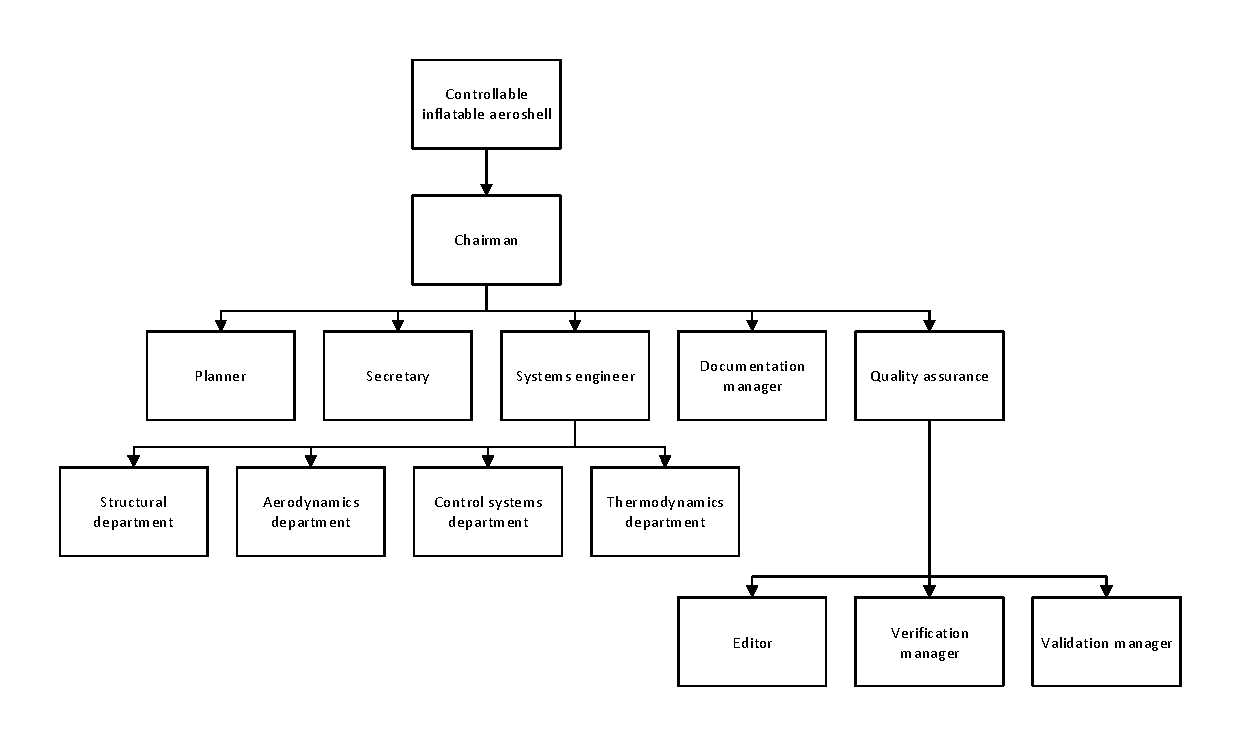
\includegraphics[width=0.95\textwidth]{./Figure/OBS.pdf}
\caption{Organisational breakdown structure} \label{fig:OBS}
\end{figure}

\subsection{Management breakdown}\label{subsec:management}
% Organisational Breakdown Structure (organogram with the responsibilities of the various group members)
The size of the project group, with nine people, is too large to be self-organizing: if no organizational structure is apparent, people will not have a clear view of the required work, leading to inefficient time-management. Therefore the organization is broken down into different positions with corresponding responsibilities. All positions do not entail exclusive contribution of the appointed functions, but indicate where final responsibility lies for each aspect. Therefore team members assist and communicate with one another between different management functions.


\subsubsection{Chairman}\label{subsec:Chairman}
The size of the DSE project group, with 9 people, is too large to be self-organizing: if no organizational structure is apparent, people will not have a clear view of the required work, leading to inefficient time-management. The role of the chairman is to prepare team meetings and guide them such that the meeting itself is performed in an efficient manner, but also the goal of the meeting is achieved: at the end of the meeting, all team members should have a clear overview of the current status of the project, as well as their present responsibilities. It is the task of the chairman to guide meetings such that this information is conveyed between the team members including the members responsible for planning, documentation, and the system engineer. Concretely, this also encompasses making the agenda.

\subsubsection{Secretary}\label{subsec:Secretary}
	The secretary shall minute during both project and customer meetings and keep track of design decisions and how they are made. This is done to assure that changes in the design process can be reviewed and remember why changes are made the way they are made. Furthermore, the secretary shall be responsible for all internal and external communication.

\subsubsection{Documentation manager}\label{subsec:D_and_A}
One of the tasks of the documentation manager is to maintain a structure in the file system used on the computer (i.e. keeping Dropbox and Github organized). The documentation manager is also the person to set up the initial files (like the LaTeX templates) and folder structures. The documentation manager should provide basic rules for the layout of the documents, communication with the editor is needed when the layout does not conform these rules. It is needed that this structure is maintained throughout the project and group members should make an effort to keep it this way, if not it is the documentation manager that will point out these problems towards the group and come with possible solutions. 

\subsubsection{Planner}\label{subsec:Planner}
The planner provides an overview for all the work packages as progressing through to time in the form of a Gantt chart. It is the function of the planner to frequently update and further detail this chart throughout the progress of the project. Furthermore more the planner is required to communicate all deadlines to the group members. Interactions between different tasks are provided and planning is made accordingly to allow all tasks to be finished before the set deadlines or milestones. Progression is recorded throughout the process to ascertain that all deadlines are met. 



\subsubsection{Systems engineer}\label{subsec:SE}
The systems engineer is responsible for the overall technical progress of the project. He keeps track of the project requirements and manages the interfaces between different design disciplines. His responsibilities can be summarized as follows:

\begin{itemize}
\item Track project requirements and overall technical progress
\item Manage design interfaces between design disciplines
\item Resolve design conflicts due to conflicting requirements 
\end{itemize}


\subsubsection{Risk Engineer}\label{subsec:RiskEng}
To mitigate cost or time overruns or even worse, eventual product failure, risk management plays a central role within project management. In order to properly address the risks involved in developing an inflatable aeroshell one person is ultimately responsible for possible hazard management: The risk engineer. The task of this risk engineer is to manage the various risks encountered during the design process. This will be done by using technical budgeting to manage the performance risks during the various design phases. Performance margins can be defined for each system and subsystem that influence the performances of other systems. In addition to this risk mapping will be used. By identifying critical components of each proposed concept and allocating the available resources accordingly the project risks can be minimized. Risk management is a continuous process.

\subsubsection{Quality assurance}\label{subsec:QA}
\paragraph{Editor}
Primary function is assuring consistent and high quality of all written communication, by means of proof-reading and correcting of pieces submitted by all group members. In addition, the lay-out and structure of reports and presentations is scrutinized and egalized. Strong interaction takes place with all group members with direct contributions to the written work, while open communication with documentation manager is maintained to resolve issues with the formatting of reports. In case of repeated errors by group members, the editor makes an effort to enter conversation with the repeaters in order to identify the origin of the problem and if need be to take pre-emptive action against future occurrences.
\paragraph{Verification}
Verification occurs at multiple stages of the design. For one, concepts should be verified to check whether the developed product meets the requirements. The team member in charge of verification

\paragraph{Validation}
IEEE defines validation as ''The assurance that a product, service, or system meets the needs of the customer and other identified stakeholders. It often involves acceptance and suitability with external customers.''(ref. ''IEEE V\&V.pdf'') The person in charge of validation is thus responsible for the compliance of the product with the requirements imposed by the costumers and stakeholders. Another task is to assure that the subsystem requirements contribute to accomplishing the system requirements and in the end to the top level requirements.


\subsection{Engineering breakdown}\label{subsec:engineer}
The engineering work of the controllable inflatable aeroshell is divided into different departments. These departments are the driving fields in the design of an inflatable aeroshell and will cover all aspects of the design. As for the management positions, engineering departments are not isolated in the sense that the aim is to involve team members in multiple design aspects.

\subsubsection{Aerodynamics department}\label{subsec:aero}
The aerodynamics department will look at different shapes possible to do the entry in the Martian atmosphere. This department looks at the hypersonic aerodynamics and determines the amount of thermal energy the heat shield needs to absorb and the loads that the structure needs to endure. In addition, the creation of a aerodynamic model of the vehicle that will be used in the control system is produced by the aerodynamics department.

\subsubsection{Structures department}\label{subsec:struct}
The structures department is responsible for the design of the structure, carrying primarily the mechanical and thermal loads by aerodynamic forces and heating. This design entails appropriate material selection, design and sizing of load-carrying elements and integrating the design while maintaining feasibility in terms of manufacturability, costs and weight. For the purpose of determining structural performance, the structures department is responsible for the development of structural tools. Moreover, the structures department actively communicates with other departments to synthesize the system design.

\subsubsection{Control systems department}\label{subsec:control}
The control systems department will analyze the controllability and stability, both static and dynamic, of the vehicle. Further this department will design the subsystems that will provide the needed characteristics for the controllability and stability. The control department covers all additional subsystems to ensure a controllable and stable vehicle, i.e. an attitude determination system.

\subsubsection{Thermal control department}\label{subsec:therm}
The thermodynamics department will look at the thermal aspect of the inflatable aeroshell. The aerodynamics department will provide a boundary condition for the heat propagation within the structure. This heat propagation will be dependent on material properties and structure shape as defined by the structures department. Furthermore, the space vehicle should have thermal control such that systems can operate and humans can survive.
\section{Work Definition and Division}
This chapter treats identification and sequencing of activities required during the project and allocation of resources to these activities. As such, it comprises a Work Breakdown Structure (WBS) and Work Flow Diagram (WFD) as primary Systems Engineering elements to categorize respectively sequence work activities. In addition, the WFD provides interrelations between steps to identify iterations in the work process where appropriate. It is essential that work activities are defined and sequenced in order to allocate resources, as depicted by the Gantt chart.

This chapter is structured as follows. The first section commences with a presentation of the WBS and accompanying discussion to justify the categorization, the second section proceeds with a presentation of the WFD, the third section discusses allocation of resources and presents the Gantt chart. The latter is accompanied by a brief discussion on milestones set to monitor project progress.

\subsection{Work Breakdown Structure}\label{sec:WBS}
Project work has been divided into a number of phases: project planning, literature research, mission analysis, tool development and enhancement, conceptual design of a first set of concepts, detailed design of a number of selected concepts and project close-out. This high-level work division is summarized firstly in the WBS displayed in Figure \ref{fig:wbs}. Whereas the sequence of activities is illustrated by the WFD, the WBS provides a categorization of activities. 

\begin{sidewaysfigure}[ht]
    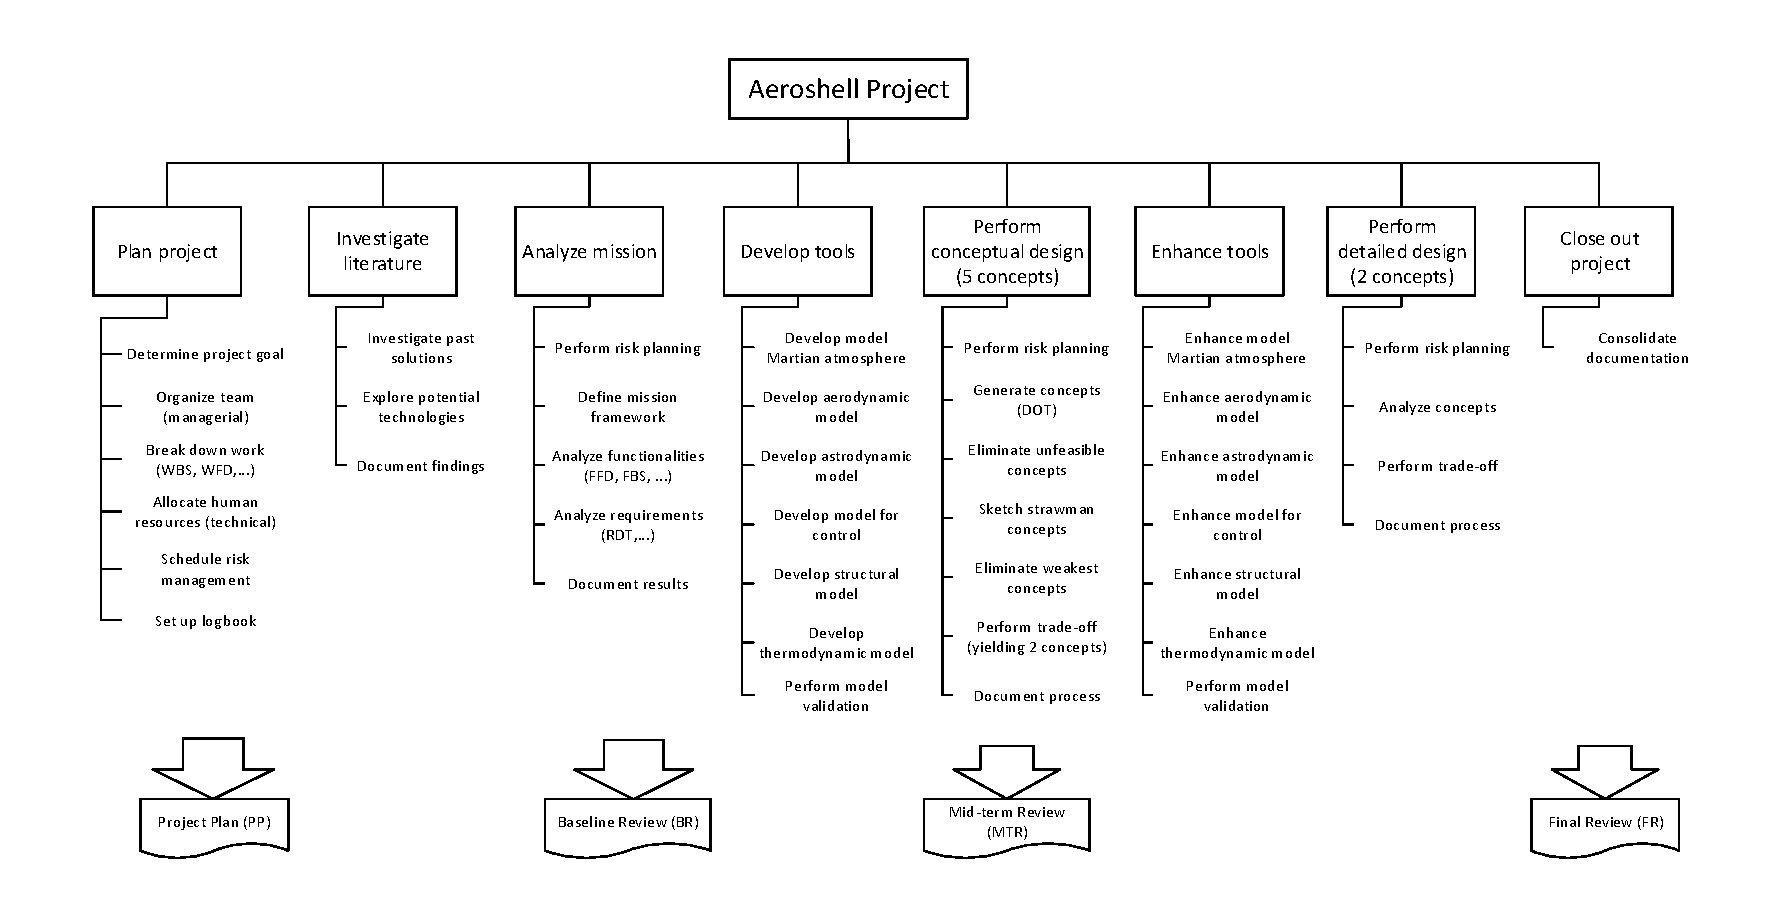
\includegraphics[scale=0.7]{Figure/WBS.pdf}
    \caption{Work Breakdown Structure (WBS) of project.}
    \label{fig:wbs}
\end{sidewaysfigure}

\subsection{Work Flow Diagram}\label{sec:WFD}
The WFD, depicted in Figure \ref{fig:wfd} elaborates on the activities depicted in the WBS (Figure \ref{fig:wbs}) and places them in a sequence. It therefore provides the basis for the allocation of human resources, as done in the Gantt chart, where all sequenced activities are placed in a timeline that fit project constraints in terms of human resources and schedule. Moreover, the WFD provides a graphical means by which to determine activities throughput and to identify iteration loops. 

\begin{sidewaysfigure}[ht]
    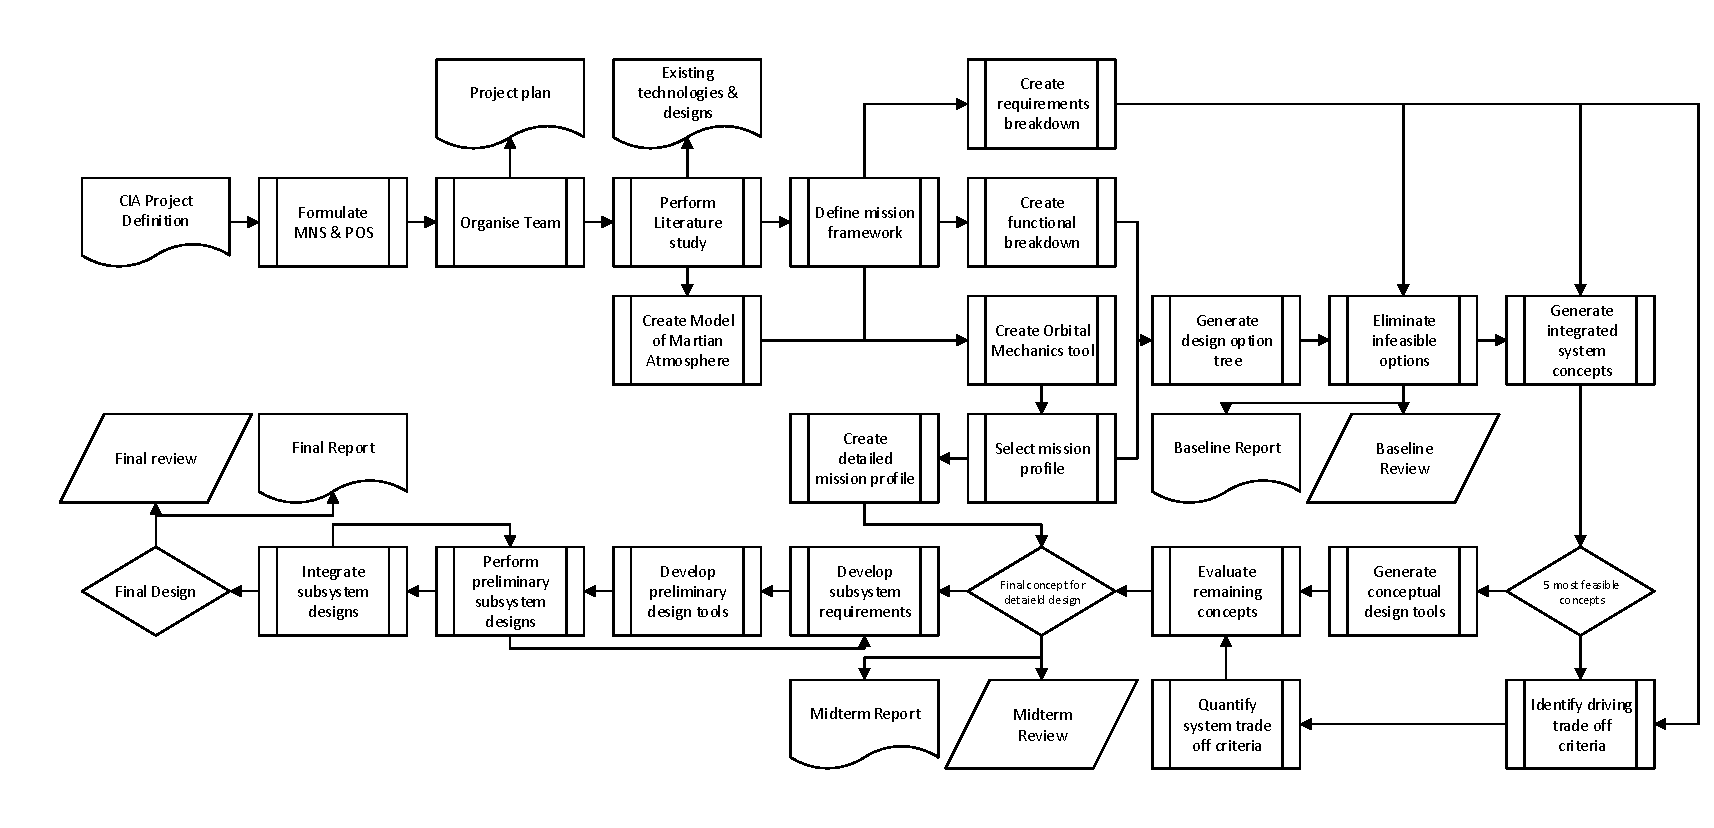
\includegraphics[scale=0.7]{Figure/WFD2.pdf}
    \caption{Work Flow Diagram (WFD) of project.}
    \label{fig:wfd}
\end{sidewaysfigure}

Lastly, it specifies identifiable milestones that close activities and project phases. Predominantly, these milestones are the following:
\begin{itemize}
\item The Project Plan (PP) finalizes provisional planning of the project, comprising: technical and managerial function appointment to team members, allocation of resources, break-down and sequencing of project work, formulation of a risk management plan and a plan for sustainable development, set-up of archiving, doucmentation and logbook and consolidating a set of project procedures.
\item The Baseline Review (BR) (and accompanying Baseline Report) finalize(s) the mission analysis phase by a liaison with the customer for agreement on mission definition, requirements and planning as well as a presentation of initial concepts formulated in the conceptual design phase.
\item The Mid-Term Review (MTR) (and accompanying Mid-Term Report) finalize(s) the first phase of concept selection, reviewing the concepts for trade-off, the trade-off process and resulting final concepts for further evaluation.
\item Final Review (FR) (and accompanying Final Report) finalize(s) the phase of concept selection with a technical presentation and agreement with the customer on the final design and the process by which it was reached. 
\end{itemize}

\subsection{Time Allocation}\label{sec:timeallocation}

A final work structure is given in the planning Gantt chart in which the time allocation for the work packages is displayed. The Gantt chart is given in figure \ref{fig:GanttChart} and provides a structured overview of the work to be done, together with allocated time slots and resources. It can be noted that the level of detail decreases as time progresses or milestones are passed. This is in line with the increasing uncertainty about the project outcomes. Based on the design choices made around the milestones different work has to be done and resources may be allotted differently. Moreover the organizational breakdown will be altered halve way based on performance so far. Resource allotment is done before the start of each phase. Some work is fixed and is indifferent to design choices made. This work, typically in the form of required deliverables is already allocated time slots in the Gantt Chart. The updating of the Gantt chart based on these design milestones in the different design phases and is the work of the planner. This planner function also includes the progress tracking in the Gantt chart as also stated in chapter \ref{cha:OBS}.

Work is typically allocated to finish a day or more before the milestones. This allows for contingency as well as an optimal functioning of the quality assurance.




\section{Project planning}\label{cha:plan}
% Schedule of the OS design project, indicating the project phasing and the planning for the delivery of the items presented in a bar chart

\subsection{Risk mitigation plan}
\label{sec:riskmit}
During the course of this project several risks are present. The risk of a certain occurrence is defined as the product  In order to prevent schedule overruns and guarantee the technical performance of the system to be designed these risks will have to be identified and managed properly. This will be done with the methods discussed in the subsequent sections.

\subsubsection{Risk mapping}
During the conceptual design phase the elements of each of the concepts to be considered will be included in a risk map. From this risk map a comparison between the risks involved in the different conceptual designs can be made. First the elements of each concept will be identified. Secondly these will be included into the risk map. This risk map consists of a table with on the X-axis the consequence of failure of each element. These are rated qualitatively from low to high as 'negligible', 'marginal', 'critical' or 'catastrophic'. \\
\noindent Negligible consequences barely influence the functioning of the system. Marginal consequences present inconveniences in performing the design mission, possibly with a small reduction in technical performance. However, the system will still be able to complete its primary mission with some (minor) adjustments. System performance is only severely compromised when a critical or catastrophic failure occurs. Critical failures strain the capabilities of the system and make mission succes questionable. A degradation in technical performance is to be expected. Catastrophic failure causes immediate mission failure or severely compromises the technical performance of the system. 
\noindent On the Y-axis the current state of the technology of each element is presented. It is assumed during risk identification that this technology state is interchangeable with the probability of failure of the element. The technology states are rated as either 'feasible in theory', 'working laboratory model', 'based on existing non-flight engineering', 'extrapolated from existing flight design' or 'proven flight design'. Elements and technologies that have only been proven as 'feasible in theory' have an inherently higher probability of failure than a component that has already been proven to function during flight.
\noindent From this risk mapping table it can be seen that the elements that present the greatest hazards for mission completion are those whose failure is either critical or catastrophic and whose technology has not matured enough yet, e.g. has only been proven in theory or has not functioned outside of a laboratory situation yet. To mitigate the risks these elements pose during the different design phases the fraction of resources allocated to 

\subsubsection{Technical budgetting}
\section{Approach with respect to sustainable development}\label{cha:sustain}
Sustainable development in engineering means that the design, production, operation and disposal of a product should be done in a sustainable way. In this case sustainable means that energy and resources are used in a manner that does not threaten the environment or the needs of future generations. In this chapter the general approach with respect to the sustainable development of the controllable inflatable aeroshell is briefly discussed.

Even though sustainability is becoming more important in engineering, it is of less importance in these kind of space missions. The reason for this is that the proposed mission is a single mission and therefore its total impact will be relatively small. For example, it is acceptable that the production of the space vehicle is less sustainable than the production of one small passenger aircraft, since the aircraft is produced in large numbers whereas only one space vehicle is produced. It can therefore be said that sustainability will not be the design driver for the controllable inflatable aeroshell. Of course, sustainable methods are preferred when they do not add much costs and very unsustainable methods are to be avoided.

Some examples of sustainable methods can be mentioned. In the process of producing the aeroshell unnecessary polluting methods that threaten the natural environment should be avoided. Also interplanetary forward contamination should be prevented. In this case it means that life and other forms of contamination should not be transferred from Earth to Mars. In practice this is already standard procedure. Another, less important, form of sustainability is the avoidance of space debris in the atmospheres of Earth and Mars.

Therefore sustainability will not be a leading driver for the design of the controllable inflatable aeroshell, as long as very unsustainable methods are avoided. The latter is effected by a preference of sustainable methods in choices for production and operation of the aeroshell.
\section{Conclusion}\label{cha:conclusion}

\subsection{Requirements}
In this section the top-level requiremets are stated. They can be found in table \ref{tab:requirements}.

\begin{table}[H]
	\caption {Requirement}
    \begin{tabular}{|l|l|}
    \hline
    Code          & Description                                                                                                      \\ \hline
    CIA-Sys-A01-1 & The re-entry vehicle shall be able to cope with an entry velocity of seven kilometers per second.                \\ \hline
    CIA-Sys-A01-2 & The inflated aeroshall shall have a maximum diameter of 12 meters.                                               \\ \hline
    CIA-Sys-A01-3 & The diameter of the launcher fairing shall be 5 meters.                                                          \\ \hline
    CIA-Sys-A01-4 & The maximum entry mass of the re-entry vehicle shall be 10,00 kilograms.                                         \\ \hline
    CIA-Sys-A01-5 & The hypersonic deceleration system mass shall not be havier than ten percent of the total re-entry vehicle mass. \\ \hline
    CIA-Sys-A01-6 & The control system shall have a maximum failure probability of 5.0e-4.                                           \\ \hline
    CIA-Sys-A01-7 & The maximum allowable loads on the re-entry vehicle shall be 3 earth g's in each axis                            \\ \hline
    CIA-Sys-A01-8 & The re-entry vehicle shall have a maximal aerobraking duration of ten days.                                      \\ \hline
    \end{tabular}
    \label{tab:requirements}
\end{table}



\subsection{System description}


% Bibliography
\newpage
\bibliography{./Bibliography/Bibliography}
\bibliographystyle{ieeetr}
% Appendix
\newpage
\begin{appendices}
\section{Project Gantt Chart}

\begin{sidewaysfigure}[ht]
    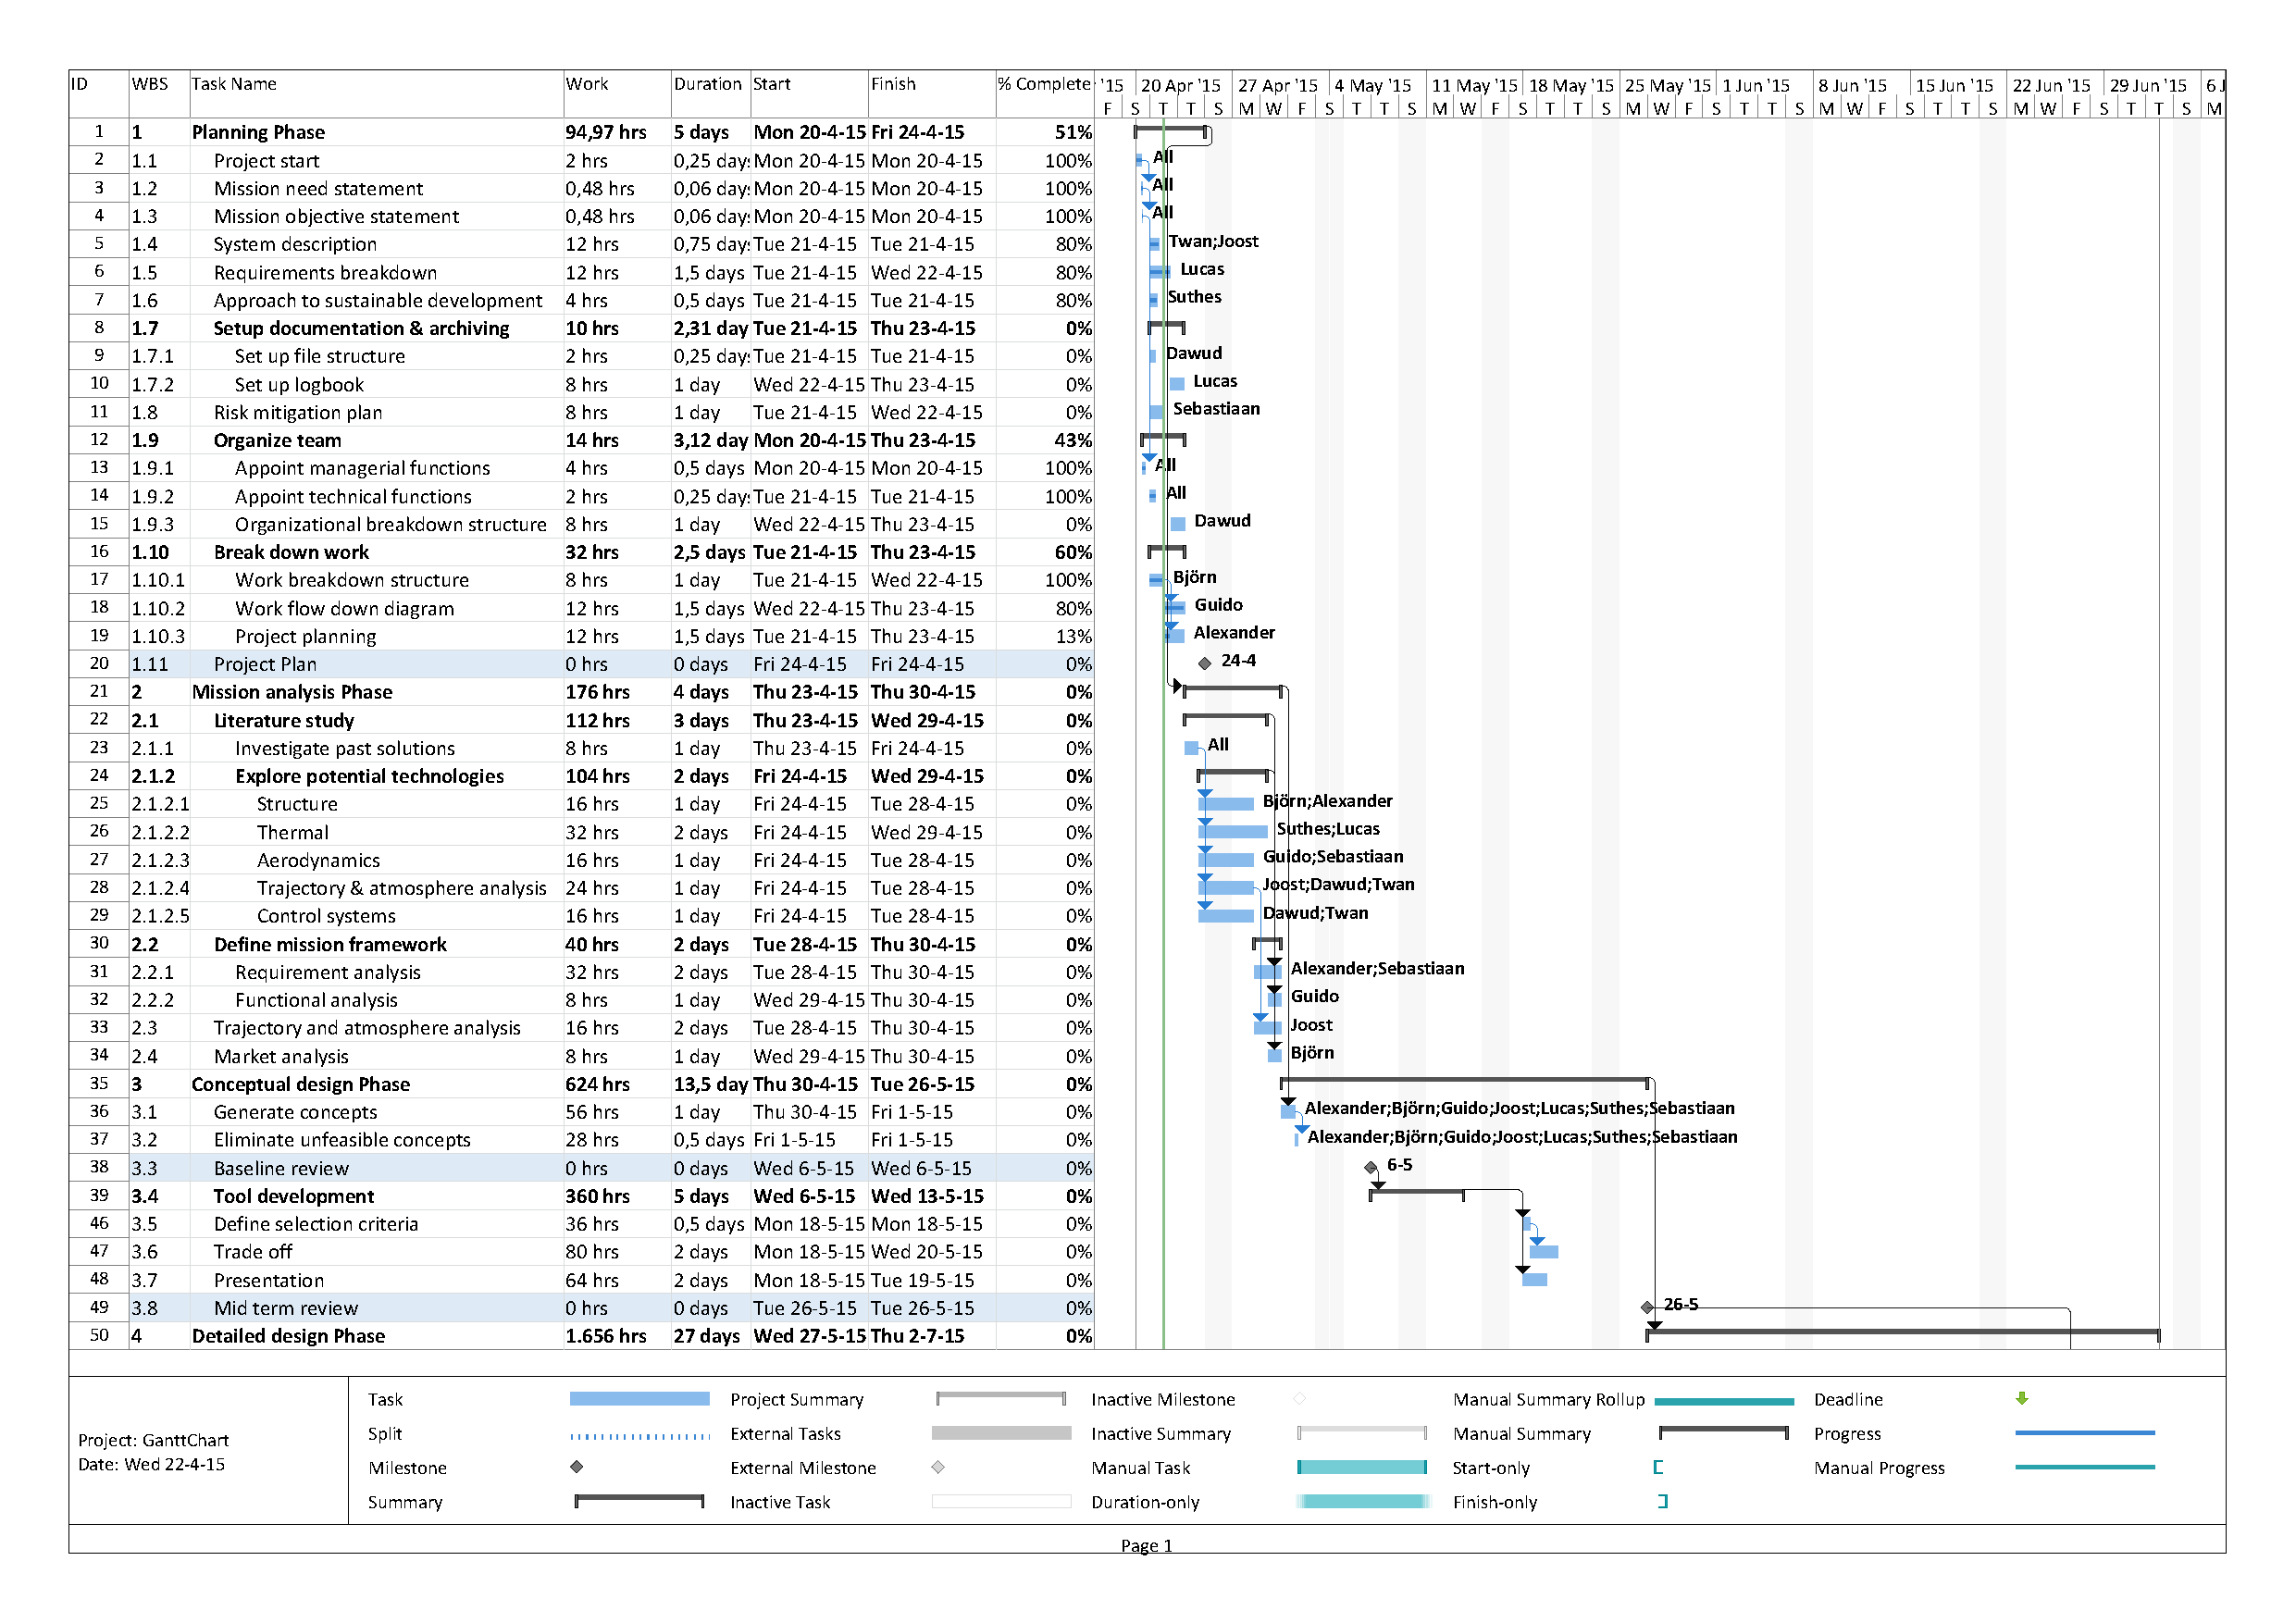
\includegraphics[scale=0.9]{Figure/GanttChart.pdf}
    \caption{Project planning}
    \label{fig:GanttChart}
\end{sidewaysfigure}

\begin{sidewaysfigure}[ht]
    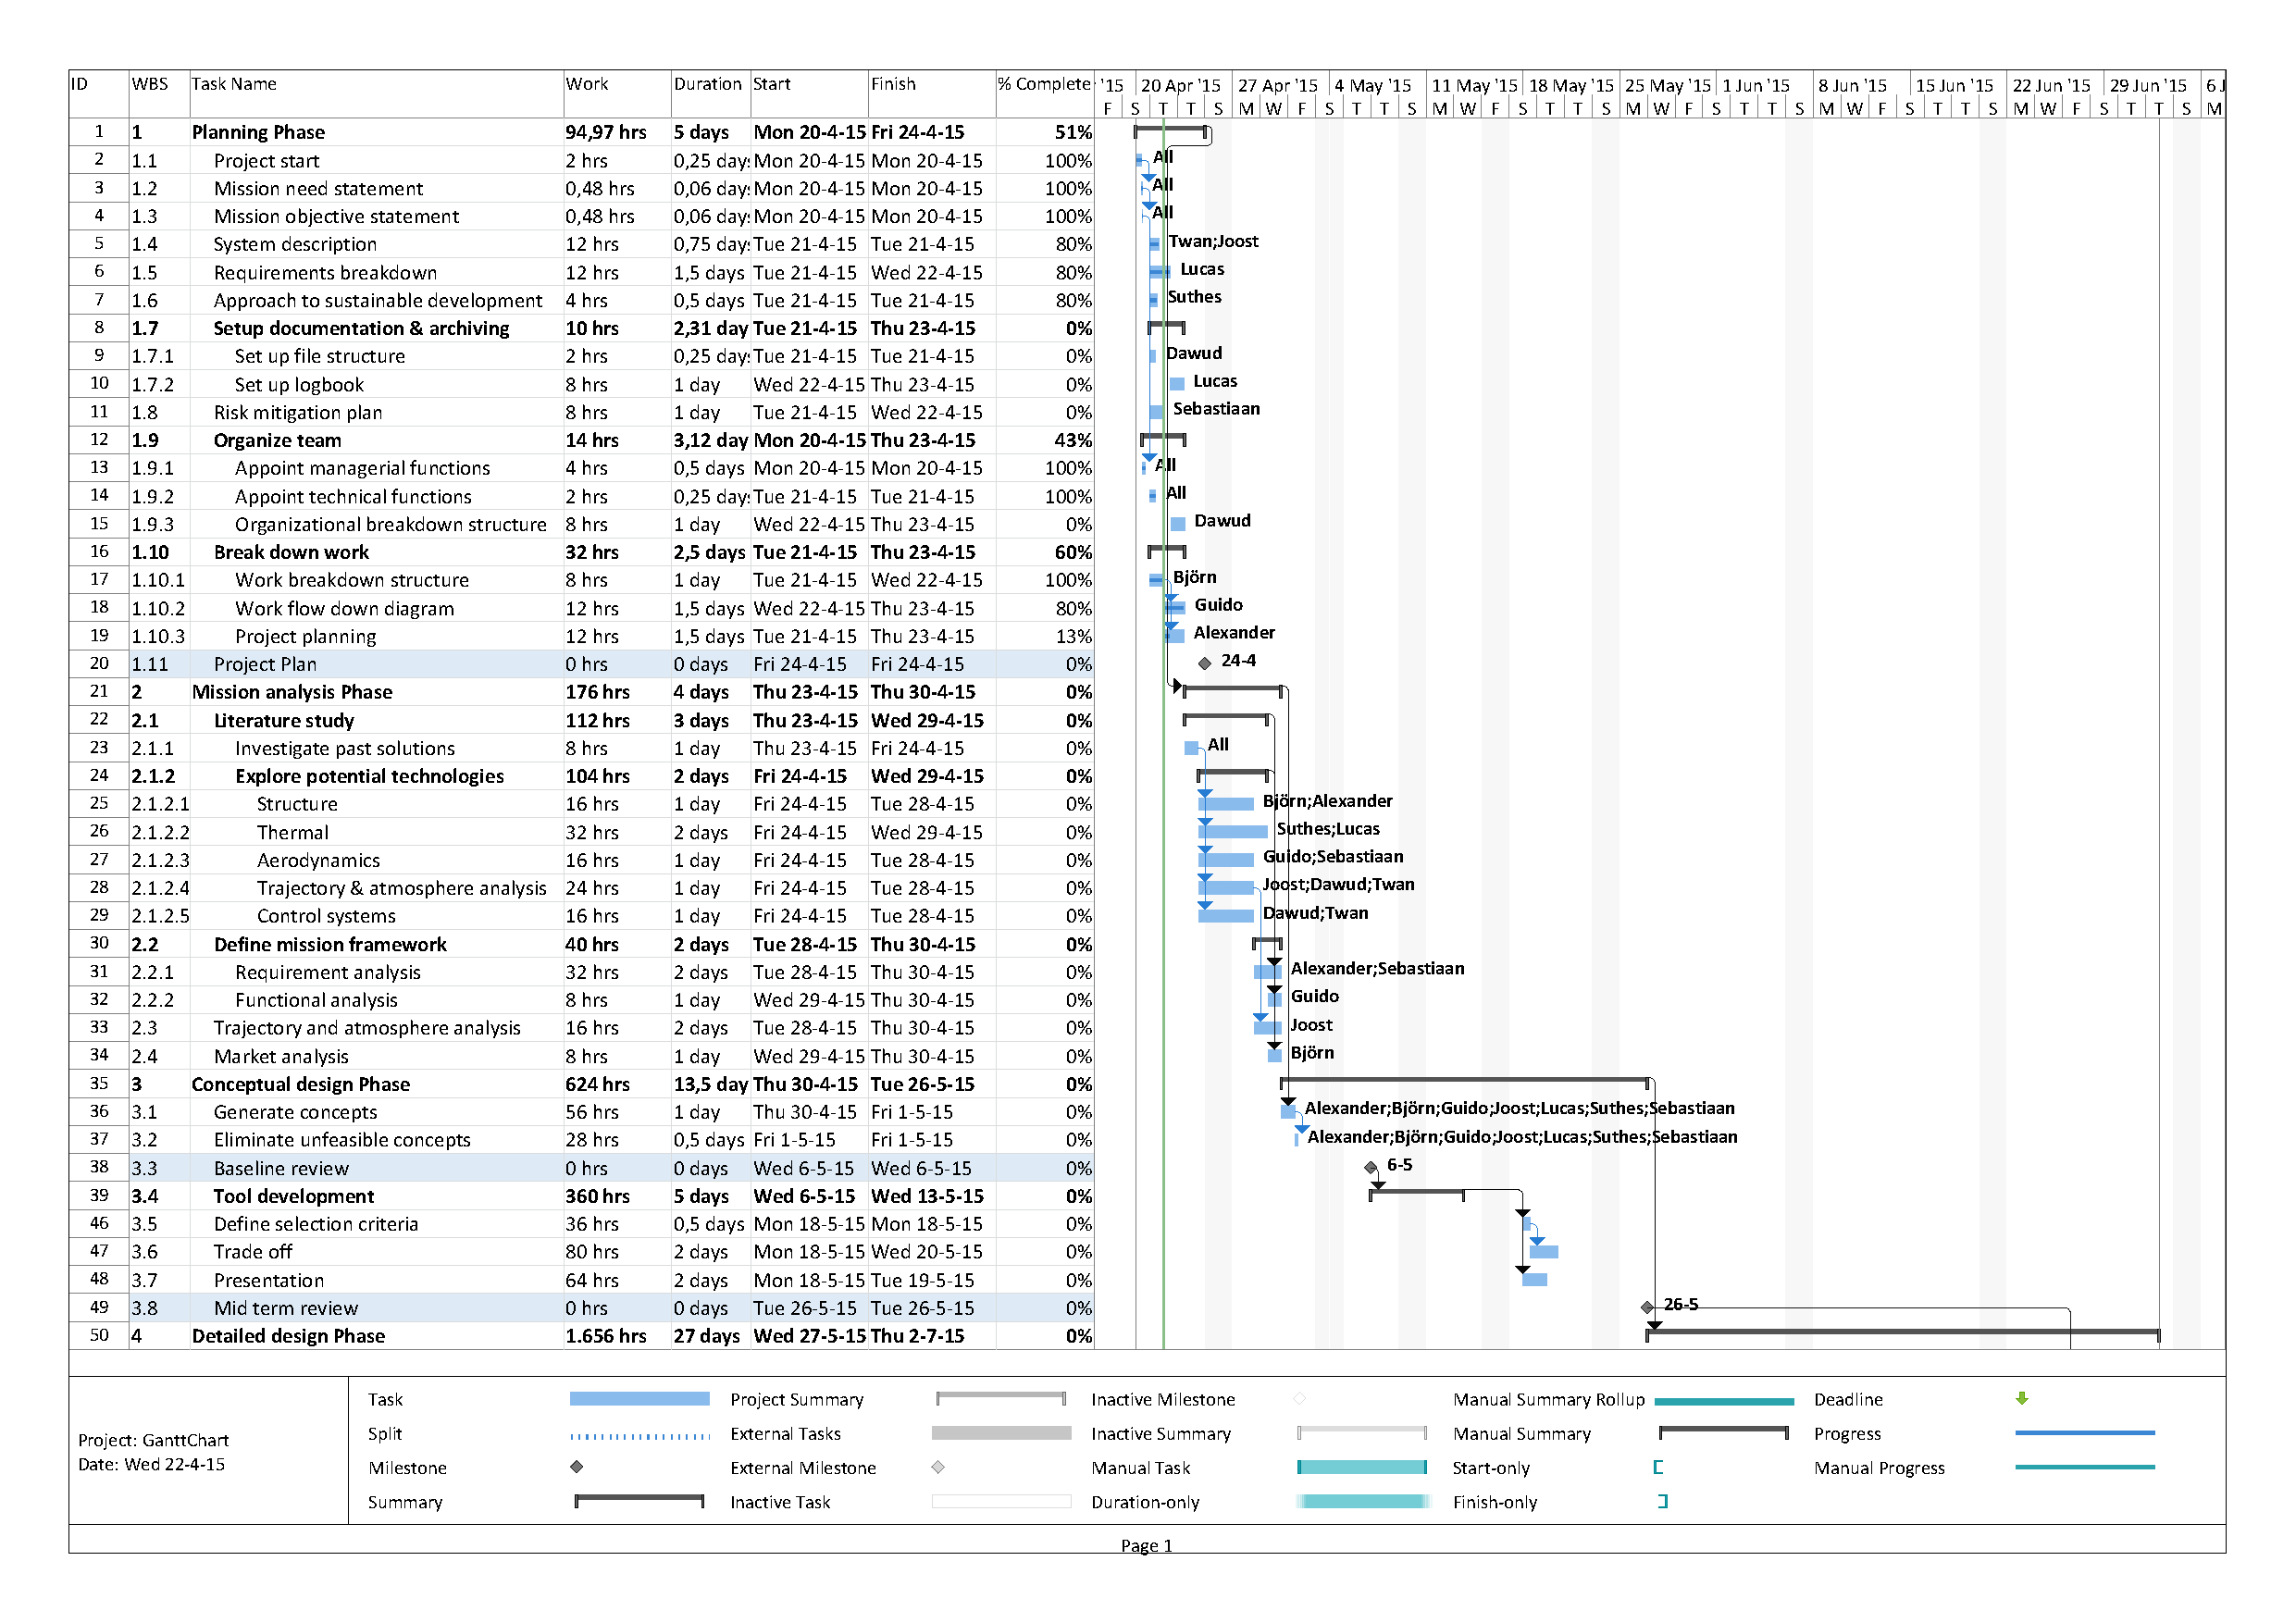
\includegraphics[scale=0.9]{Figure/GanttChart.pdf}
    \caption{Project planning}
\end{sidewaysfigure}

\end{appendices}
\end{document}